%%%%%%%%%%%%%%%%%%%%%%%%%%%%%%%%%%%%%%
%%  
%% chapter 4: Device Parallelism
%%
%%%%%%%%%%%%%%%%%%%%%%%%%%%%%%%%%%%%%%

\def\ArtDir{04.DevPar/figures}%


\chapter{Device parallelism}
\label{chapter:parallelism}

\begin{itemize}
  \item So far learnt how to transfer execution to the device.
  \item Also know how to get some memory to the device.
  \item But not expressed any parallelism on the device yet.
  \item This is the focus here: running in parallel on a target device.
  \item Firstly introduce the hierarchical view of parallelism, with three levels, then move onto loop which needs teams.
  \item This chapter will go through them in detail.
  \item Crucial to remain strictly in OpenMP terminology: the target is still an abstract device (GPU).
  \item We {\bf do not} talk about how OpenMP teams/threads/simd map to GPU specific things like work-items/work-groups/compute units etc. That will come in Chapter~\ref{chapter:portable}.
\end{itemize}


\section{The goal: teams distribute parallel for simd}
\begin{itemize}
  \item Remind the readers we're heading towards the full directive.
\end{itemize}

\section{Teams}
\label{sec:teams}
\begin{itemize}
  \item We know about teams from the host.
  \item Threads are launched in a team.
  \item Allowed to synchronize threads in a team with barrier.
  \item Explain barrier if not already done in Chapter~\ref{chapter:overview}.
  \item May have multiple teams, a league of teams.
  \item num\_teams clause to target directive.
  \item num\_threads clause for threads in a team. Multiplicative factor.
  \item Disclaimer: clauses specifying numbers not good style. See Chapter~\ref{chapter:portable}.
  \item But need to know about multiple teams having one or more threads.
  \item Execution so far is master thread in each team executes the code in the target region.
\end{itemize}

\subsection{teams distribute}
\label{ssec:teams_distribute}
\begin{itemize}
  \item Workshare loop iterations between teams.
  \item Only master thread in each time executes.
  \item dist\_schedule clause.
\end{itemize}


\subsection{teams API functions}
\label{ssec:teams_query_functions}

\section{parallel}
\begin{itemize}
  \item Parallelism for threads in each team.
  \item Will apply to all teams.
\end{itemize}

\subsection{parallel for}
\begin{itemize}
  \item Workshare loop iterations between threads in a team.
  \item Interaction with the teams distribute: iterations distributed in chunks by teams, then iterations of chunk workshared between threads.
  \item Combined directive: teams distribute parallel for
\end{itemize}

\section{simd}
\begin{itemize}
  \item Each thread executes SIMD instructions.
  \item Must be applied to a loop.
  \item Compiler will vectorize it.
  \item Be careful, because this doesn't behave the same as worksharing depending on the nesting.
  \item See the Beyond OpenMP book for more details.
\end{itemize}

\section{teams distribute parallel for simd}
\label{sec:bud}
\begin{itemize}
  \item Use the combined directive to show parallelism of a big loop.
  \item Compiler and runtime will deal with mapping and distribution of work.
  \item Very similar to loop if you let compiler choose the distribution which you should.
\end{itemize}

\section{Example: Parallel vector add}
\begin{itemize}
  \item Take vector add from previous chapter.
  \item Arrays still on stack (no map clauses).
  \item Keep the data on the stack so don’t have to do the data movement? Means we can do all the data movement together later.
  \item Example shows adding parallelism using teams distribute parallel for simd.
\end{itemize}

\section{Examples: Batched DGEMM}
\begin{itemize}
  \item Shows example of hierarchical parallelism.
  \item Compute one matrix per team, using multiple threads.
  \item Recommend using linear algebra libraries, this is a motivating example.
\end{itemize}

\section{The loop directive}
\label{sec:loop}
\begin{itemize}
  \item Introduce the loop directive.
  \item Good for one big parallel loop.
  \item Challenges of the semantics of nested loop directives - suggest to avoid doing it on the target.
  \item The spectrum of prescriptive vs descriptive.
  \item What if you need more control? What happens underneath in OpenMP? Lead into next sections.
  \item Mention loop collapse clause is not mechanical collapse, applies loop semantics to the loop nest.
  \item Mention it's teams loop, to split up creation of parallelism with the concurrency of the loop.
  \item BUT we need teams first, so loop has to come after.
  \item Explore semantic differences around synchronization and implicit parallel regions with this example:
\end{itemize}

\begin{Verbatim}
#pragma omp target teams loop
for (int i = 0; i < N; ++i) {
  // .. do something per team
  #pramga omp loop bind(parallel)
  for (int j = 0; j < M; ++j) {}
}

#pragma omp target teams distribute
for (int i = 0; i < N; ++i) {
  // .. do something per team
  #pramga omp parallel for simd
  for (int j = 0; j < M; ++j) {}
}
\end{Verbatim}


%-----------------------------------------------------------------------
%------------------------- From Next Step ------------------------------
%-----------------------------------------------------------------------
\section{From The Next Step Chapter 6}
\subsection{The Target Teams Construct}
\label{sec:06.teams-construct}
\index{OpenMP constructs!Target teams}
\index{Accelerators!Target teams}
\index{Accelerators!League}
\index{Accelerators!Initial thread}

Strictly speaking, \code{target teams} is a combined construct made up of the
\code{target} and \code{teams} constructs.  But since a
\code{teams} construct may appear only nested immediately inside a
\code{target} construct with no other intervening statements or declarations
between the two constructs, the two constructs are inseparable.
The \code{teams} construct syntax in C/C++ and Fortran is shown in
Figure~\ref{figure:syntax-teams-construct}.

\begin{figure}[!tb]
\centering
\begin{tabular}{|l|}
\hline
\ompbcteams \ompclauses  \\
\hspace{2em}\emph{structured block} \\
\hline
\ompbfteams \ompclauses \\
\hspace{2em}\emph{structured block} \\
\ompbfteamsend \\
\hline
\end{tabular}
\caption{ \textbf{Syntax of the teams construct in C/C++ and Fortran} -- \small
          Create a league of initial threads each in its own team.
          }
\label{figure:syntax-teams-construct}
\end{figure}

Similar to the \code{parallel} construct, the \code{target}~\code{teams} construct 
specifies that the subsequent code block should be run in parallel.
A \code{parallel} construct creates a team of threads, where the thread
that encountered the \code{parallel} construct becomes the master thread.  Each
thread in the team executes the parallel region.  
The \code{target}~\code{teams} construct starts a \emph{league} of initial
threads where each thread is in its own team.  Each initial thread executes the
teams region in parallel (see Section~\ref{ssec:06.contention-groups}).  One
can think of the \code{target} construct as a \code{target}~\code{teams}
construct that creates a league with only one initial thread.

%Work-sharing constructs, such
%as the loop construct, control how the threads in a team share the execution of
%code in the parallel region.
%As shown in Figure~\ref{figure:chapter6-teams-mxv}, 

\index{Accelerators!League}
When a \code{parallel}
construct is encountered by a league, each thread in the league becomes the
master of a new team of threads. The result is a league of teams where each
team has multiple threads.  Each team of threads concurrently executes the
parallel region.  

The clauses that may appear on
the \code{teams} construct are listed in Figure~\ref{figure:syntax-teams-clauses}.  
Clauses from both the \code{target}
and \code{teams} constructs may appear on the The \code{target}~\code{teams}
construct.  

\index{OpenMP clauses!num\_teams}
\index{OpenMP clauses!thread\_limit}
\index{OpenMP clauses!default}
\index{OpenMP clauses!private}
\index{OpenMP clauses!firstprivate}
\index{OpenMP clauses!shared}
\index{OpenMP clauses!reduction}
\index{Accelerators!Num\_teams clause}
\index{Accelerators!Thread\_limit clause}
\index{Accelerators!Default clause}
\index{Accelerators!Private clause}
\index{Accelerators!Firstprivate clause}
\index{Accelerators!Shared clause}
\index{Accelerators!Reduction clause}
\begin{figure}[!htbp]
\centering
\begin{tabular}{|l l|}
\hline
\bcnumteams & (C/C++)\\
\bfnumteams & (Fortran)\\
\bcthreadlimit & (C/C++)\\
\bfthreadlimit & (Fortran)\\
\bcdefault & (C/C++)\\
\bffdefault & (Fortran)\\
\bprivate & \\
\bfirstprivate & \\
\bshared & \\
\breduction & \\
\hline
\end{tabular}
\caption{ \textbf{Clauses supported by the teams construct} -- \small
          The \texttt{num\_teams} and \texttt{thread\_limits} clauses are 
          described below.
          }
\label{figure:syntax-teams-clauses}
\end{figure}

\index{Accelerators!Contention group}\index{Contention group}
The number of teams created by a \code{target}~\code{teams} construct is
implementation defined or is specified by the \code{num_teams} clause.  Each
team is executing in its own contention group.  The maximum number of threads
active in a contention group is specified by the \code{thread_limit} clause.  

What is the real difference between the \code{target}~\code{teams} and
\code{parallel} constructs? Both constructs fork multiple threads that execute
the subsequent block of code in parallel.  The \code{target teams} construct is
asserting a more restricted form of parallelism than the \code{parallel}
construct allows.  The compiler can take advantage of these restrictions and be
much more aggressive at exploiting parallelism.  These restrictions are as
follows:

\begin{itemize}

  \item Because the teams that are started by a \code{target teams}
  construct are each in their own contention group, threads from different 
  teams cannot synchronize with each other.

  \item The only \OMP\ constructs that can appear in a \code{teams} region
  are the \code{parallel}, \code{distribute} and any other \code{parallel} or
  \code{distribute} regions arising from related constructs.  These are
  listed here: \begin{itemize}
      \item \code{parallel} 
      \item \code{parallel for} (C/C++)
      \item \code{parallel do} (Fortran)
      \item \code{parallel sections}
      \item \code{distribute} 
      \item \code{distribute simd}
      \item \code{distribute parallel for} (C/C++)
      \item \code{distribute parallel do} (Fortran)
      \item \code{distribute parallel for simd} (C/C++)
      \item \code{distribute parallel do simd} (Fortran)
  \end{itemize}

\end{itemize}

\index{Accelerators!League}
\index{Accelerators!Initial thread}
In Figure~\ref{figure:chapter6-teams-v1} the \code{target}~\code{teams} construct
at line $6$ creates a league of initial threads.  Each initial thread is in its own team.
The initial threads (and therefore the teams) are numbered from $0$ to $N-1$ where
$N$ is the number of initial threads created.  The number of inital threads
is returned by the \OMP\ runtime function \code{omp_get_num_teams}.
\index{Accelerators!omp\_get\_num\_teams}
\index{OpenMP runtime functions!omp\_get\_num\_teams}

\begin{figure*}[!tb]
\begin{verbatim}
 1 #include <omp.h>
 2 extern void do_team_work(int, int, int, int);
 3 #pragma omp declare target(do_team_work)
 4 void f()
 5 {
 6   #pragma omp target teams
 7   {
 8     int team = omp_get_team_num();
 9     int nteams = omp_get_num_teams();
10     int tid = omp_get_thread_num(); // Always 0
11     int nthreads = omp_get_num_threads(); // Always 1
12     do_team_work(team, nteams, tid, nthreads);
13   } // End of target teams
14 }
\end{verbatim}
\caption{ \textbf {Example of the target teams construct } -- \small
          Multiple initial threads execute the function \texttt{do\_team\_work()}.     
         }
\label{figure:chapter6-teams-v1}
\end{figure*}

Calling the \code{omp_get_team_num()} in a teams region returns the team
number of the initial thread.  Since each team is a single intial thread, the calls to
\code{omp_get_num_threads()} at line $11$ and \code{omp_get_thread_num()} at line $10$
will always return one and zero, respectively. 
\index{Accelerators!omp\_get\_team\_num}
\index{OpenMP runtime functions!omp\_get\_team\_num}
\index{Accelerators!omp\_get\_num\_threads}
\index{OpenMP runtime functions!omp\_get\_num\_threads}
\index{Accelerators!omp\_get\_thread\_num}
\index{OpenMP runtime functions!omp\_get\_thread\_num}

Each initial thread calls the function \code{do\_team\_work()} at line $12$ passing in
the team number, the number of teams, the thread number and the number of threads in the
team.  Figure~\ref{figure:chapter6-teams-pic} diagrams the execution of the
region assuming four initial threads.

\begin{figure*}[!tbh]
\centering
\pdfimageresolution 400
\fbox{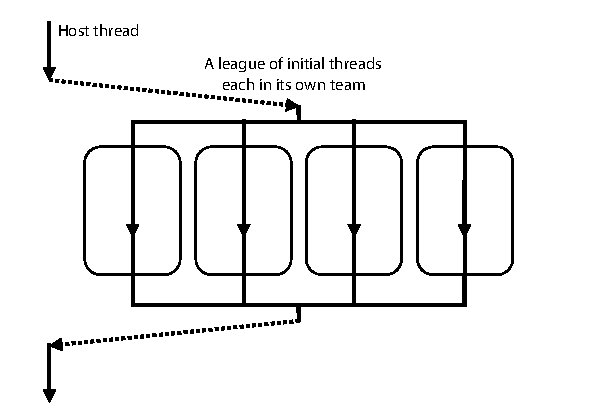
\includegraphics[clip=true,scale=1.00]
         {\ArtDir/device-teams1.pdf}
     }
\caption{ \textbf{The target teams construct creates a league of initial 
               threads} -- \small
        Each initial thread is a team of one thread.  The inital threads
        execute the teams region in parallel.
        }
\label{figure:chapter6-teams-pic}
\end{figure*}

\index{Accelerators!League}
\index{Accelerators!Initial thread}
In Figure~\ref{figure:chapter6-teams-v2}, the \code{target}~\code{teams} construct again
creates a league of initial threads, but this time each initial thread
immediately encounters the \code{parallel} construct at line $7$. Each initial thread then
becomes the master of a new team of multiple threads.  The number of teams and
a thread's team number are determined by the \code{omp_get_num_teams} and
\code{omp_get_team_num} runtime functions, respectively.
\index{Accelerators!omp\_get\_team\_num}
\index{OpenMP runtime functions!omp\_get\_team\_num}
\index{Accelerators!omp\_get\_num\_teams}
\index{OpenMP runtime functions!omp\_get\_num\_teams}

\begin{figure*}[!tbh]
\begin{verbatim}
 1 #include <omp.h>
 2 extern void do_team_work(int, int, int, int);
 3 #pragma omp declare target(do_team_work)
 4 void f()
 5 {
 6   #pragma omp target teams num_teams(4)
 7   #pragma omp parallel num_threads(5)
 8   {
 9     int team = omp_get_team_num();
10     int nteams = omp_get_num_teams();
11     int tid = omp_get_thread_num();
12     int nthreads = omp_get_num_threads();
13     do_team_work(team, nteams, tid, nthreads);
14   } // End of target teams
15 }
\end{verbatim}
\caption{ \textbf {Example of a parallel construct nested in a 
                   target teams construct} -- \small
          Multiple teams of threads execute the function \texttt{do\_team\_work()}.     
         }
\label{figure:chapter6-teams-v2}
\end{figure*}

The call to the \code{omp_get_num_threads()} function at line $12$ returns the
number of threads in a team, which is $5$. The call to \code{omp_get_thread_num}
at line $11$ returns the threads number in the range $0$ to $4$.
Each thread in each team (a total of 20 threads) then calls the function
\code{do\_team\_work()} passing in the team number, the number of teams, the thread number and
the number of threads in the team.  Figure~\ref{figure:chapter6-teams-pic2} diagrams
the execution of all the threads, assuming four teams with five threads per
team.

Note that if the thread calling \code{omp_get_team_num} is in a team that was
initiated by a parallel region nested inside a teams region, the function still
returns the number of the initial thread that is the ancestor of the thread.

\index{Accelerators!League}
\begin{figure*}[!tbh]
\centering
\pdfimageresolution 400
\fbox{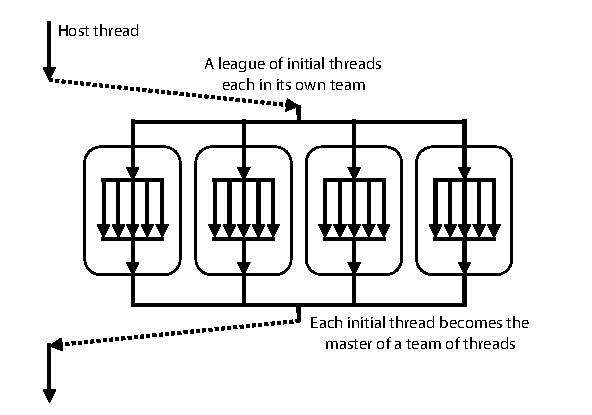
\includegraphics[clip=true,scale=1.00]
         {\ArtDir/device-teams2.pdf}
     }
\caption{ \textbf{The initial threads created by the teams construct each
               become the master of a new team of threads.  } -- \small
        Each initial thread starts execution as team of one thread.  The initial threads
        execute the teams region in parallel and immediately encounter
        a parallel construct.  Each initial thread then becomes the
        master of a new team of threads.
        }
\label{figure:chapter6-teams-pic2}
\end{figure*}

%-----------------------------------------------------------------------
%------------------------- New subsection ------------------------------
%-----------------------------------------------------------------------
\subsection{The Distribute Construct}
\label{ssec:06.distribute-construct}
\index{OpenMP constructs!Distribute}
\index{Accelerators!Distribute}

\index{Accelerators!League}
\index{Accelerators!Initial thread}
The \code{target}~\code{teams} construct starts a league of initial threads where each
thread is in its own team.  Similar to the loop construct, the
\code{distribute} construct is a worksharing construct that distributes
the iterations of a loop to the initial threads in a league.  The loop
iterations are divided into chunks, which are then scheduled across the initial
threads in a league.

The \code{distribute} construct syntax in C/C++ and Fortran is shown in
Figure~\ref{figure:syntax-distribute-construct}.

\begin{figure}[!htb]
\centering
\begin{tabular}{|l|}
\hline
\ompbcdistribute \ompclauses  \\
\hspace{2em}\emph{for-loops} \\
\hline
\ompbfdistribute \ompclauses \\
\hspace{2em}\emph{do-loops} \\
\ompbfdistributeend \ompclauses \\
\hline
\end{tabular}
\caption{ \textbf{Syntax of the distribute construct in C/C++ and 
               Fortran} -- \small
          Distribute loop iterations to the initial threads in
          a league.
          }
\label{figure:syntax-distribute-construct}
\end{figure}

The clauses that are available on
the \code{distribute} construct are listed in Figure~\ref{figure:syntax-distribute-clauses}.  

\index{OpenMP clauses!private}
\index{OpenMP clauses!firstprivate}
\index{OpenMP clauses!lastprivate}
\index{OpenMP clauses!collapse}
\index{OpenMP clauses!dist\_schedule}
\index{Accelerators!Private clause}
\index{Accelerators!Firstprivate clause}
\index{Accelerators!Lastprivate clause}
\index{Accelerators!Collapse clause}
\index{Accelerators!Dist\_schedule clause}
\begin{figure*}[!tbh]
\centering
\begin{tabular}{|l|}
\hline
\bprivate \\
\bfirstprivate \\
\blastprivate \\
\bcollapse \\
\bdistschedule \\
\hline
\end{tabular}
\caption{ \textbf{Clauses supported by the distribute 
               construct} -- \small
          The dist\_schedule clause is described below.
          }
\label{figure:syntax-distribute-clauses}
\end{figure*}

Variables that appear in the \code{private}, \code{firstprivate} or
\code{lastprivate} clause are private in each initial thread.
The \code{distribute} construct has no implicit barrier at the end of the
construct.  This is like having a loop construct with a \code{nowait} clause.
The initial threads do not synchronize at a barrier at the end of the region.

The \code{collapse} clause has the same behavior as it does on the loop
construct.  It collapses the iterations of perfectly nested loops into a single
iteration space.
The restrictions on the format of the loop to which the construct applies are
the same as those for the loop construct.

How the loop iterations are scheduled to execute across the initial threads in
the league is implementation-defined, unless the \code{dist_schedule} clause is
present.
When the \code{dist_schedule(static)} clause is present, the loop iterations
are divided into contiguous chunks. If \emph{chunk\_size} appears in the
clause, then it specifies the size of the chunks.  Otherwise, each thread is
assigned no more than one chunk, and the chunks are roughly equal in size.

\index{Accelerators!League}
A version of the familiar saxpy (single precision $y=a*x+y$) function is
shown in Figure~\ref{figure:chapter6-distribute-v1}.  The \code{distribute}
worksharing construct distributes the iterations of the loop to the
initial threads in the league started by the \code{target teams} construct.

\begin{figure*}[!tb]
\begin{verbatim}
1 void saxpy(float *restrict y, float *restrict x, float a, int n)
2 {
3   #pragma omp target teams map(y[:n]) map(to:x[:n]) 
4   #pragma omp distribute
5   for (int i=0; i<n; i+=n)
6   {
7       y[i] =  y[i] + a*x[i];
8   }
9 }
\end{verbatim}
\caption{ \textbf {Example of the distribute worksharing construct} -- \small
          Each initial thread created by the target teams construct 
          executes a subset of the iterations in the loop's iteration space.
         }
\label{figure:chapter6-distribute-v1}
\end{figure*}

What is the difference between the execution of the \code{for} (or \code{do} in Fortran) and the
\code{distribute} worksharing constructs? The \code{distribute} construct has the potential
for better performance because of the restrictions on where it can be used and
what other \OMP\ constructs can appear inside the distribute region.  This
enables the compiler to be more aggressive with optimizations.  The
\code{for} and \code{do} constructs are more versatile but may not perform as well.  

The idea behind the \code{target}~\code{teams} and \code{distribute} constructs is to
spread the execution of a loop coarsely across hardware compute units and
then more finely to the threads that execute within those compute units.  What
we have shown so far is how to distribute the loop iteration to the compute
units.

The code in Figure~\ref{figure:chapter6-distribute-v2} converts the saxpy loop
into a doubly nested loop.  

\begin{figure*}[!tbh]
\begin{verbatim}
 1 void saxpy(float *restrict y, float *restrict x, float a, int n)
 2 {
 3   // Assume n is even
 4   #pragma omp target teams map(y[:n]) map(to:x[:n]) num_teams(2) 
 5   #pragma omp distribute
 6   for (int j=0; j<n; j+=n/2)
 7   {
 8     #pragma omp parallel num_threads(4)
 9     #pragma omp for
10     for (int i=j; i<n/2; i++)
11       y[i] = y[i] + a*x[i];
12   }
13 }
\end{verbatim}
\caption{ \textbf {Example of worksharing a loop across two levels of
                   parallelism} -- \small
          Use team level parallelism on the outer loop and thread level
          parallelism on the inner loop.  Distribute the loop iterations to two
          teams.  Each team then uses four threads to execute the iterations
          that are assigned to it.  
         }
\label{figure:chapter6-distribute-v2}
\end{figure*}

\index{Accelerators!League}
\index{Accelerators!Initial thread}
The \code{distribute} construct at line $5$ assigns the execution of two
iterations in the outer loop to a league of two initial threads.  The
\code{parallel} construct at line $8$ is then encountered by each initial
thread with different values for \code{j}.  Each initial thread becomes the master
thread in a team of four threads.  The first team executes the first half of
the loop iterations and the second team executes the other half.  The loop
iterations scheduled to execute on an initial thread are then scheduled
according to the \code{for} worksharing construct at line $9$, to execute on
the team of threads that the initial thread is now the master of.

In accelerated worksharing, loops are first scheduled at a coarse level to
teams and then more finely to the threads in each team.  We rewrote the saxpy
loop in order to schedule it across two levels of parallelism: teams and
threads.  However, rewriting loops is tedious and is something we want to avoid.

Section~\ref{ssec:06.composite-worksharing-loop-construct} introduces
\emph{composite} accelerated worksharing constructs.  When composite
accelerated worksharing constructs are used, loop itertions are distributed
across multiple levels of parallelism without having to rewrite the loop as we
did in Figure~\ref{figure:chapter6-distribute-v2}.  

%-----------------------------------------------------------------------
%------------------------- New subsection ------------------------------
%-----------------------------------------------------------------------
\subsection{Combined and Composite Accelerated Worksharing Constructs}
\label{ssec:06.composite-worksharing-loop-construct}
\index{Composite construct}
\index{Combined construct}
\index{Combined construct! Target}
\index{Combined construct! Target teams}
\index{Accelerators!Workshare construct}

Recall that combined constructs are short-hand notation for specifying the
individual constructs in which one construct is immediately nested inside another.
For example, the \code{parallel}~\code{for} combined construct is equivalent to
a \code{parallel} construct with a \code{for} construct nested immediately
inside the \code{parallel} construct.  The combined construct has the same
execution behavior as the two separate constructs.  However, in some instances,
depending on the compiler, the combined constructs may achieve better
performance than the individual constructs.

With some exceptions, the clauses that may appear on a combined
construct are any of the clauses that may appear on the individual
constructs that make up the combined construct.
There are many new combined
constructs involving the device constructs.  They are presented
in this section in two groups.  

The first group is the \emph{combined target} constructs.  The constructs in
this group combine the \code{target} construct with other constructs.
The second group is the \emph{combined target teams} constructs.  
They combine the \code{target teams} construct with new
worksharing constructs.  This second group is discussed at the end of this section
after the new worksharing constructs are presented.

The syntax for the combined target constructs in C/C++ and Fortran
are shown in Figure~\ref{figure:chapter6-combined-target}.  The combined
target constructs that include a \code{parallel} directive create a
team of threads where the initial thread is the master of the team.
The target simd region is executed by an initial thread that uses SIMD
parallelism to execute the iterations of the subsequent loop.

\index{OpenMP constructs!Target parallel}
\index{Accelerators!Target parallel}
\index{OpenMP constructs!Target parallel loop}
\index{Accelerators!Target parallel loop}
\index{OpenMP constructs!Target parallel loop simd}
\index{Accelerators!Target parallel loop simd}
\index{OpenMP constructs!Target simd}
\index{Accelerators!Target simd}
\begin{figure}[!htbp]
\centering
\begin{tabular}{|l|}
\hline
\ompbctargetparallel \ompclauses \\
\hspace{2em}\emph{structured block} \\
\hline
\ompbctargetparallelfor \ompclauses \\
\hspace{2em}\emph{for-loops} \\
\hline
\ompbctargetparallelforsimd \ompclauses \\
\hspace{2em}\emph{for-loops} \\
\hline
\ompbctargetsimd \ompclauses \\
\hspace{2em}\emph{for-loops} \\
\hline
\hline
\ompbftargetparallel \ompclauses \\
\hspace{2em}\emph{structured block} \\
\ompbftargetparallelend \ompclauses \\
\hline
\ompbftargetparalleldo \ompclauses \\
\hspace{2em}\emph{do-loops} \\
\ompbftargetparalleldoend \ompclauses \\
\hline
\ompbftargetparalleldosimd \ompclauses \\
\hspace{2em}\emph{do-loops} \\
\ompbftargetparalleldosimdend \ompclauses \\
\hline
\ompbftargetsimd \ompclauses \\
\hspace{2em}\emph{do-loops} \\
\ompbftargetsimdend \ompclauses \\
\hline
\end{tabular}
\caption{ \textbf{Syntax of the combined target constructs in C/C++ and Fortran} -- \small
          Constructs combining \texttt{target} with other constructs.  A \texttt{copyin}
          clause may not appear on any of the combined target constructs.
          }
\label{figure:chapter6-combined-target}
\end{figure}

A composite construct is different than a combined construct.  
Composite constructs combine multiple constructs, but the combination has
execution behavior that is different from when the constructs are specified
separately.  

\index{Accelerators!League}
\index{Accelerators!Initial thread}
The \code{distribute}~\code{parallel}~\code{for} construct is a composite
accelerated worksharing construct that distributes the iterations of a loop
across two levels of parallelism.  Each initial thread in the league that
encounters the construct becomes the master thread of a team.  The iterations
of a loop are first distributed to the master threads.  The subset of loop
iterations assigned to the master thread are then again distributed to the
threads in the team.

The code in Figure~\ref{figure:chapter6-distribute-v3} shows how the
~\code{distribute}~\code{parallel}~\code{for} accelerated worksharing
construct is used to distribute the iterations of the saxpy loop to 
teams and then to the threads in those teams.

Another way to look at this type of construct is to consider the nested version
of the C/C++ saxpy loop from Figure~\ref{figure:chapter6-distribute-v2}.  We had
to rewrite the loop to distribute its iterations across two levels of
parallelism.

The \code{distribute}~\code{parallel}~\code{for} (or
\code{distribute}~\code{parallel}~\code{do} in Fortran) construct tells the
compiler to create the second level of parallelism and to distribute loop
iterations across the two levels of parallelism.  So, now we don't have to
rewrite loops!

\begin{figure*}[!tbh]
\begin{verbatim}
1 void saxpy(float *restrict y, float *restrict x, float a, int n)
2 {
3   #pragma omp target teams map(y[:n]) map(to:x[:n]) 
4   #pragma omp distribute parallel for
5   for (int i=0; i<n; i++)
6     y[i] = y[i] + a*x[i];
7 }
\end{verbatim}
\caption{ \textbf {Example of the distribute parallel loop accelerated 
                   worksharing construct} -- \small
          Create multiple thread teams executing in parallel.
          Distribute loop iterations to the teams and then
          to the threads in each team.
         }
\label{figure:chapter6-distribute-v3}
\end{figure*}

\index{Accelerators!League}
\index{Accelerators!Initial thread}
The first level of parallelism is created by a \code{target}~\code{teams} construct.  When
the resulting league of initial threads encounters
the \code{distribute}~\code{parallel}~\code{loop} construct, the following steps occur:
\begin{enumerate}

\item By the \code{distribute} part of the construct, each initial thread is
assigned loop iterations according to the \code{distribute} construct's
scheduling algorithm.

\item By the \code{parallel} part of the construct, each initial thread becomes
the master thread of a thread team.  This creates the second level of
parallelism. Now multiple teams of threads are
executing in parallel.

\item By the \code{for} part of the construct, the subset of iterations
assigned to each initial thread (the master thread) are then distributed across
the threads in each team.

\end{enumerate}

The composite accelerated worksharing constructs and their syntax in C/C++ and
Fortran are shown in Figure~\ref{figure:chapter6-accel-work-sharing-construct}.
With a few exceptions, all clauses that may appear on the individual directives
that make up the construct, may appear on the composite construct.

\index{OpenMP constructs!Distribute parallel loop}
\index{Accelerators!Distribute parallel loop}
\index{OpenMP constructs!Distribute simd}
\index{Accelerators!Distribute simd}
\index{OpenMP constructs!Distribute parallel loop simd}
\index{Accelerators!Distribute parallel loop simd}
\begin{figure}[!htbp]
\centering
\begin{tabular}{|l|}
\hline
\ompbcdistributeparallelfor \ompclauses  \\
\hspace{2em}\emph{for-loops} \\
\hline
\ompbcdistributesimd \ompclauses  \\
\hspace{2em}\emph{for-loops} \\
\hline
\ompbcdistributeparallelforsimd \ompclauses  \\
\hspace{2em}\emph{for-loops} \\
\hline
\hline
\ompbfdistributeparalleldo \ompclauses \\
\hspace{2em}\emph{do-loops} \\
\ompbfdistributeparalleldoend \ompclauses \\
\hline
\ompbfdistributesimd \ompclauses \\
\hspace{2em}\emph{do-loops} \\
\ompbfdistributesimdend \ompclauses \\
\hline
\ompbfdistributeparalleldosimd \ompclauses \\
\hspace{2em}\emph{do-loops} \\
\ompbfdistributeparalleldosimdend \ompclauses \\
\hline
\end{tabular}
\caption{ \textbf{Syntax of the composite accelerated worksharing constructs 
               in C/C++ and Fortran} -- \small
          Distribute loop iterations across multiple levels of
          parallelism: teams, threads and SIMD lanes.
          }
\label{figure:chapter6-accel-work-sharing-construct}
\end{figure}

The \code{distribute}~\code{simd} construct distributes loop iterations across
two levels of parallelism.  Loop iterations are assigned to the initial
threads in a league according to the \code{distribute} constructs scheduling
algorithm.  Each initial thread then uses SIMD parallelism to execute
the loop iterations assigned to it.

The \code{distribute}~\code{parallel}~\code{for}~\code{simd} (or
\code{distribute}~\code{parallel}~\code{do}~\code{simd} in Fortran)  construct
distributes loop iterations across three levels of parallelism.  Loop
iterations are first assigned to the initial threads in each team.  Each
initial thread becomes the master of a new team of threads.  The loop
iterations assigned to an initial thread are then distributed to the threads in
the master thread's team.  Each thread then uses SIMD parallelism to execute
the iterations assigned to it.

The composite accelerated worksharing constructs may be combined with the
\code{target teams} construct.  As mentioned at the beginning of this section,
these are called combined target teams constructs.  The combined target teams
constructs and their syntax in C/C++ and Fortran are shown in
Figure~\ref{figure:chapter6-combined-teams}.  
%Some of them are quite long.

\index{Combined construct!Target teams}
\index{OpenMP constructs!Target teams distribute simd}
\index{Accelerators!Target teams distribute simd}
\index{OpenMP constructs!Target teams distribute}
\index{Accelerators!Target teams distribute}
\index{OpenMP constructs!Target teams distribute parallel loop}
\index{Accelerators!Target teams distribute parallel loop}
\index{OpenMP constructs!Target teams distribute parallel loop simd}
\index{Accelerators!Target teams distribute parallel loop simd}
\begin{figure}[!htbp]
\centering
\begin{tabular}{|l|}
\hline
\ompbctargetteamsdistribute \ompclauses \\
\hspace{2em}\emph{for-loops} \\
\hline
\ompbctargetteamsdistributeparallelfor \ompclauses \\
\hspace{2em}\emph{for-loops} \\
\hline
\ompbctargetteamsdistributesimd \ompclauses \\
\hspace{2em}\emph{for-loops} \\
\hline
\ompbctargetteamsdistributeparallelforsimd{ \emph{[clause[[,]\ldots}}\\
\hspace{2em}\emph{for-loops} \\
\hline
\hline
\ompbftargetteamsdistribute \ompclauses \\
\hspace{2em}\emph{do-loops} \\
\ompbftargetteamsdistributeend \\
\hline
\ompbftargetteamsdistributeparalleldo \ompclauses \\
\hspace{2em}\emph{do-loops} \\
\ompbftargetteamsdistributeparalleldoend \\
\hline
\ompbftargetteamsdistributesimd \ompclauses \\
\hspace{2em}\emph{do-loops} \\
\ompbftargetteamsdistributesimdend \\
\hline
\ompbftargetteamsdistributeparalleldosimd \ompclauses \\
\hspace{2em}\emph{do-loops} \\
\ompbftargetteamsdistributeparalleldosimdend \\
\hline
\end{tabular}
\caption{ \textbf{Syntax of the combined target teams constructs in C/C++ and Fortran} -- \small
          Constructs that combine \texttt{target teams} and accelerated worksharing constructs.
          }
\label{figure:chapter6-combined-teams}
\end{figure}

\index{Combined construct!Target teams reduction}
Because the \code{target teams} construct is a combined construct, 
the \code{target} construct may be separated out of 
a combined target teams construct (see Section~\ref{sec:06.teams-construct}).
For example, a \code{target teams distribute} construct may be separated into a
\code{target} construct with an immediately nested \code{teams
distribute} construct.  Typically, this is simply a syntax preference, but
there are some instances when \code{target} must be a separate construct.
This can occur when a variable must be \code{private} in the teams region and
mapped in the target region.  

A variable cannot appear in both a \code{map} clause and a data-sharing
attribute clause on the same
construct.  For example, in Figure~\ref{figure:chapter6-targetteams-reduction}
the variable \code{sum} appears in a \code{reduction} clause, and therefore, cannot also
appear in a \code{map} clause.  Because \code{sum} is not mapped, its reduced value is 
lost after the \code{target teams} region completes.\footnote{The same problem
can occur when using a \code{reduction} clause on the target combined constructs.}

\begin{figure*}[!tbh]
\begin{verbatim}
 1 int dotp(int *restrict a, int *restrict b, int n)
 2 {
 3   int sum = 0;
 4 
 5   #pragma omp target teams distribute map(to:a[:n],b[:n]) \
 6                                       reduction(+:sum)
 7   for (int i=0; i<n; i++)
 8     sum += a[i] * b[i];
 9 
10   return sum;  // Sum is always 0
11 }
\end{verbatim}
\caption{ \textbf {A variable cannot appear in both map and reduction clauses on the same construct} -- \small
          The \texttt{reduction} clause is associated with the
          \texttt{teams} directive.
          The variable \texttt{sum} is not mapped, and therefore,
          the reduced value of \texttt{sum} is lost after the region.
        }
\label{figure:chapter6-targetteams-reduction}
\end{figure*}

The solution, as shown in
Figure~\ref{figure:chapter6-targetteams-reduction-v2}, is to use a separate
\code{target} construct that explicitly maps the variable \code{sum}.  Each initial
thread that executes the teams region gets a private instance of \code{sum}.  Once
the teams region is complete, the mapped \code{sum} variable contains the reduced
value.  In the map-exit phase for the target region, the reduced value
is assigned to the host's original \code{sum} variable. 

\begin{figure*}[!tbh]
\begin{verbatim}
 1 int dotp(int *restrict a, int *restrict b, int n)
 2 {
 3   int sum = 0;
 4 
 5   #pragma omp target map(sum) map(to:a[:n],b[:n])
 6   #pragma omp teams distribute reduction(+:sum)
 7   for (int i=0; i<n; i++)
 8     sum += a[i] * b[i];
 9 
10   return sum;
11 }
\end{verbatim}
\caption{ \textbf {Use a separate target construct to map reduction variables} -- \small
          The variable \texttt{sum} is private in the teams region, but now mapped
          in the target region.
        }
\label{figure:chapter6-targetteams-reduction-v2}
\end{figure*}
